\documentclass[12pt,ngerman,parskip=half]{scrreprt}

\usepackage{babel}
\usepackage{blindtext}
\usepackage{graphicx}
\usepackage{xcolor}
\usepackage{booktabs}

\usepackage{colortbl}

\author{Uwe Ziegenhagen}
\title{\LaTeX\ und Bilder}

\usepackage{hyperref}
\hypersetup{
    bookmarks=true,                     % show bookmarks bar
    unicode=false,                      % non - Latin characters in Acrobat’s bookmarks
    pdftoolbar=true,                        % show Acrobat’s toolbar
    pdfmenubar=true,                        % show Acrobat’s menu
    pdffitwindow=false,                 % window fit to page when opened
    pdfstartview={FitH},                    % fits the width of the page to the window
    pdftitle={My title},                        % title
    pdfauthor={Author},                 % author
    pdfsubject={Subject},                   % subject of the document
    pdfcreator={Creator},                   % creator of the document
    pdfproducer={Producer},             % producer of the document
    pdfkeywords={keyword1, key2, key3},   % list of keywords
    pdfnewwindow=true,                  % links in new window
    colorlinks=true,                        % false: boxed links; true: colored links
    linkcolor=blue,                          % color of internal links
    filecolor=cyan,                     % color of file links
    citecolor=green,                     % color of file links
    urlcolor=magenta                        % color of external links
}

\begin{document}
\maketitle


\tableofcontents

\listoffigures

\listoftables

\chapter{Protestische Ethik im Zeitalter des Kapitalismus}

\section{Einleitung}

Siehe Abbildung \ref{fig:katze} auf Seite \pageref{fig:katze}

\blindtext[2]

%fixe Breite
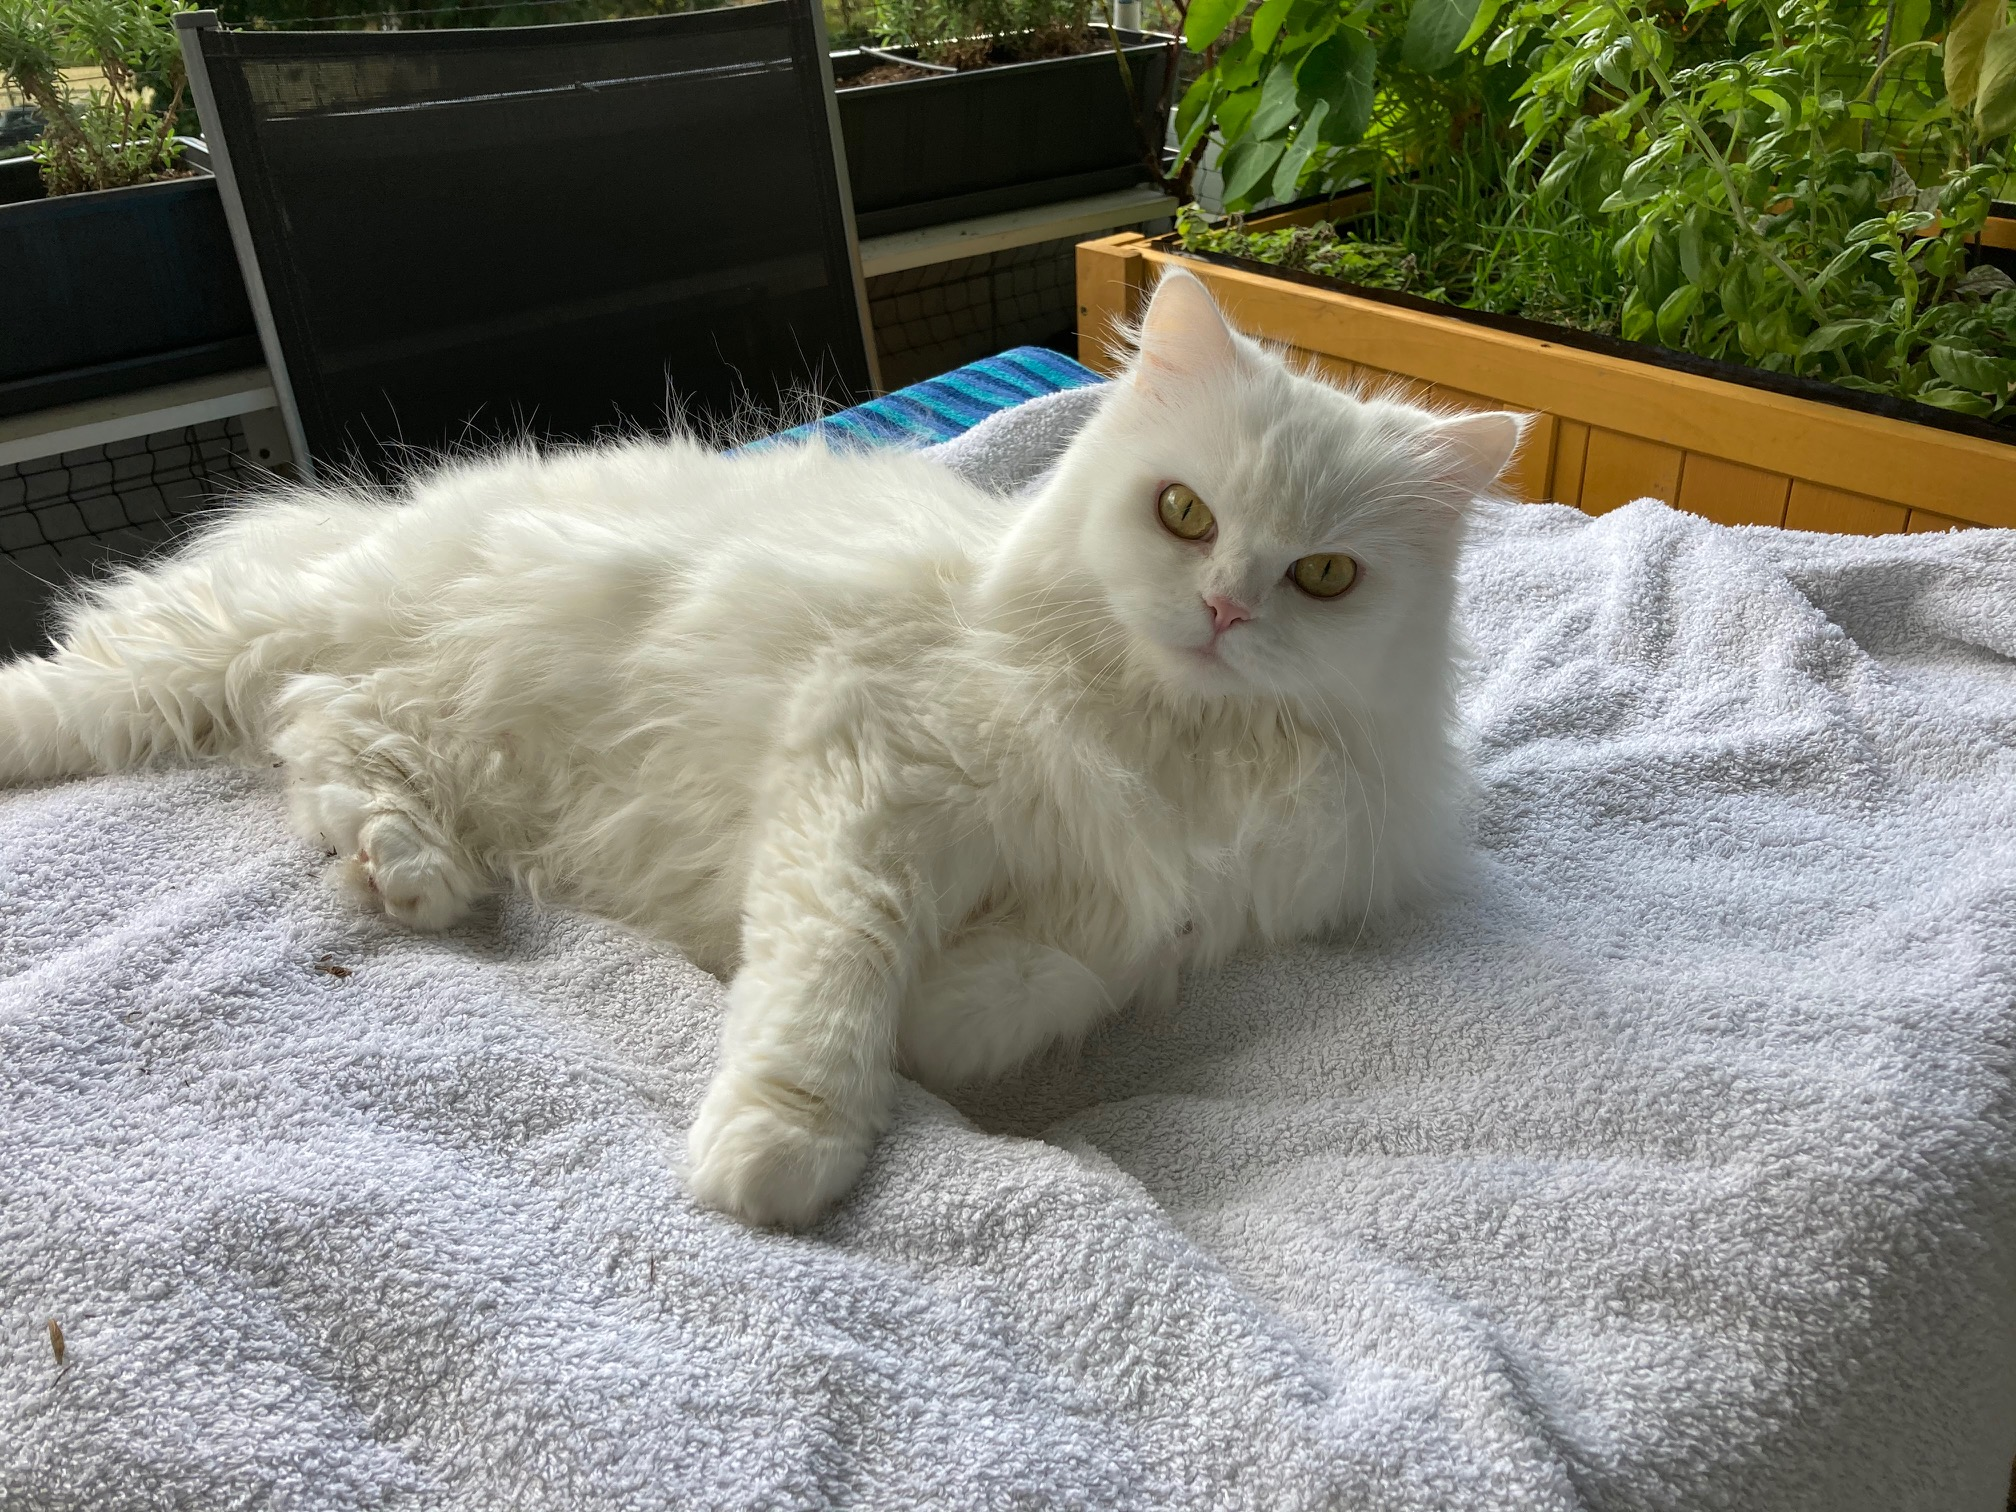
\includegraphics[width=12cm]{Bilder/Katze1}

\blindtext[2]

\section{Hauptteil}\label{sec:hauptteil}

\blindtext[2]


\begin{figure}[h]
\begin{center}

\includegraphics[width=0.9\textwidth]{Bilder/Katze}
\caption{Meine Miezekatze}\label{fig:katze}
\end{center}
\end{figure}


\blindtext[2]

\section{Fazit}\label{sec:fazit}

\blindtext[2]


\begin{figure}[h]
\begin{center}

\includegraphics[width=0.65\textwidth,angle=90]{Bilder/Katze}
\caption{Meine Miezekatze}\label{fig:katze}
\end{center}
\end{figure}


\blindtext[2]

\textbf{was fettes}

{\bfseries was fettes}


\section{Tabellen und \LaTeX}

\begin{tabular}{|l|c|r|p{6cm}|} \hline
1. Spalte & 2. Spalte & 3. Spalte & 4. Spalte \\ \hline
links & sehr zentriert&   rechts  & Ich bin ein längerer Satz in einer Tabellenspalte  \\ \hline
links & sehr zentriert&   rechts  & Ich bin ein längerer Satz in einer Tabellenspalte  \\ \hline
links & sehr zentriert&   rechts  & Ich bin ein längerer Satz in einer Tabellenspalte  \\ \hline
\end{tabular}

\section{Fließende Tabellen}

\blindtext[2]

\begin{table}
\begin{center}
\caption{Ich bin eine Tabelle}\label{tab:tabelle1}
\begin{tabular}{lcrp{6cm}} \toprule[3pt] 
\textbf{1. Spalte} & \textbf{2. Spalte} & \textbf{3. Spalte} & \textbf{4. Spalte} \\ \addlinespace[5mm] \midrule 
links & sehr zentriert&   rechts  & Ich bin ein längerer Satz in einer Tabellenspalte  \\ \midrule[1pt]
links & sehr zentriert&   rechts  & Ich bin ein längerer Satz in einer Tabellenspalte  \\ 
links & sehr zentriert&   rechts  & Ich bin ein längerer Satz in einer Tabellenspalte  \\  \bottomrule[1.5pt]
\end{tabular}
\end{center}
\end{table}



% Tabellenspalten in Standard-LaTeX
% l = linksbündig
% r = rechtsbündig
%c für zentriert
% p{Maß} Für linksbündige Absatzspalte

\blindtext[2]

% Colortbl Beispiel
 \begin{tabular}{l!{\color{green}\vrule}l}
    \arrayrulecolor{red}\hline
    test & test\\\arrayrulecolor{blue}\hline
  \end{tabular}


\end{document}

Bildformate = JPEG, PNG, PDF
